\documentclass[12pt,a4paper]{article}

\usepackage[a4paper,margin=1in]{geometry}
\usepackage{graphicx}
\usepackage{booktabs}
\usepackage{amsmath,amssymb}
\usepackage{float}
\usepackage{hyperref}
\usepackage{xcolor}
\usepackage{listings}
\usepackage{enumitem}
\usepackage{fancyhdr}
\usepackage{longtable}

\hypersetup{colorlinks=true,linkcolor=blue,urlcolor=blue}

\pagestyle{fancy}
\fancyhf{}
\lhead{ICS1512}
\rhead{Machine Learning Algorithms Laboratory}
\cfoot{\thepage}

\lstset{
language=Python,
basicstyle=\ttfamily\small,
numbers=left,
frame=single,
breaklines=true,
showstringspaces=false
}

\begin{document}

\begin{tabular}{|p{4cm}|p{11cm}|}
\hline
Experiment No. & 5 \\ \hline
Experiment Title & Decision Tree and Random Forest: A Comparative Classification Study \href{https://github.com/Kavin-ks/Machine-Learning-Projects}{\textsuperscript{1}}\\ \hline
Student Name & Kavinsoorya K S \\ \hline
Register Number & 3122247001030 \\ \hline
Faculty & Dr. Poreddy Ajay Kumar Reddy \\ \hline
Submission Date & August 16, 2026 \\ \hline
\end{tabular}

\vspace{0.5cm}

\section{Objective}
The objective of this experiment is to implement a single \textbf{Decision Tree} classifier and extend it to a \textbf{Random Forest} ensemble model to perform a comparative classification study on the Wisconsin Diagnostic Breast Cancer (WDBC) dataset. Additionally, the experiment aims to analyze the effects of critical hyperparameters (splitting criterion, maximum tree depth, minimum split samples, and minimum leaf samples for Decision Trees; and number of estimators, feature subset sizes, and bootstrapping for Random Forests) using 5-Fold Cross-Validation, select the optimal configurations, evaluate both models on an independent test set, and analyze their ability to control overfitting and improve generalization.

\section{Problem Statement}
Given a clinical dataset $\mathcal{D} = \{(\mathbf{x}_i, y_i)\}_{i=1}^n$, where $\mathbf{x}_i \in \mathbb{R}^{30}$ represents a continuous vector of features computed from a digitized image of a breast mass fine needle aspirate (FNA), and $y_i \in \{0, 1\}$ represents the clinical diagnosis of the tumor (0 for Malignant, 1 for Benign), the goal is to build machine learning models $f(\mathbf{x}) \to \{0, 1\}$ that classify tumor samples accurately. The models must maximize the classification accuracy and $F_1$-score (optimizing the trade-off between sensitivity/recall and precision) to minimize false negatives (undetected malignant tumors) and false positives (unnecessary medical interventions).

\section{Dataset Description}
The experiment is conducted using the \textbf{Wisconsin Diagnostic Breast Cancer (WDBC)} dataset from the UCI Machine Learning Repository. The dataset contains 569 samples of FNA biopsies, each characterized by 30 continuous real-valued features computed from the nuclei characteristics of the digitized images. The target variable is binary, representing the diagnosis of the tumor. Table~\ref{tab:dataset_summary} summarizes the characteristics of the dataset.

\begin{longtable}{|p{6cm}|p{8cm}|}
\hline
Dataset Name & Wisconsin Diagnostic Breast Cancer (WDBC) Dataset \\ \hline
Dataset Source & UCI Machine Learning Repository \\ \hline
Initial Sample Size & 569 records \\ \hline
Cleaned Sample Size & 569 records (0 missing values, 0 duplicate rows) \\ \hline
Number of Features & 30 continuous numerical attributes (excluding ID and Diagnosis) \\ \hline
Number of Classes & 2 (Benign: 1, Malignant: 0) \\ \hline
Missing Values & 0 (dataset contains no null entries) \\ \hline
Train-Test Split Ratio & 80\% Training (455) / 20\% Testing (114) \\ \hline
Training Class Distribution & Benign (1): 285 (62.64\%), Malignant (0): 170 (37.36\%) \\ \hline
Testing Class Distribution & Benign (1): 72 (63.16\%), Malignant (0): 42 (36.84\%) \\ \hline
\label{tab:dataset_summary}
\end{longtable}

The 30 features are computed from ten real-valued attributes of cell nuclei:
\begin{enumerate}
    \item \textbf{Geometry Metrics:} Radius (mean of distances from center to points on the perimeter), Perimeter, Area, Compactness ($\frac{\text{perimeter}^2}{\text{area}} - 1.0$).
    \item \textbf{Texture and Texture Variations:} Texture (standard deviation of gray-scale values), Smoothness (local variation in radius lengths), Symmetry, Fractal Dimension.
    \item \textbf{Boundary Shape Metrics:} Concavity (severity of concave portions of the contour), Concave Points (number of concave portions of the contour).
\end{enumerate}
For each attribute, three values are calculated: the Mean, the Standard Error (SE), and the Worst (mean of the three largest values), yielding 30 continuous features.

\section{Exploratory Data Analysis}
Exploratory Data Analysis (EDA) was performed to understand the target class distribution and evaluate pairwise correlation among features.

\subsection{Target Class Distribution}
\begin{figure}[H]
\centering

\includegraphics[width=0.7\linewidth]{images/class_distribution.png}
\caption{Target Class Distribution showing Benign (B) vs. Malignant (M)}
\label{fig:class_dist}
\end{figure}

\textbf{Inference:}
The bar chart reveals that the dataset is moderately imbalanced, with Benign (B) cases constituting approximately 62.74\% of the dataset (357 samples) and Malignant (M) cases making up the remaining 37.26\% (212 samples). Utilizing stratified sampling during the train-test split ensures that both training and testing partitions preserve this original class balance (62.64\% Benign in training, 63.16\% Benign in testing), preventing the model from becoming biased toward the majority class.

\subsection{Feature Correlation Analysis}
\begin{figure}[H]
\centering

\includegraphics[width=0.8\linewidth]{images/correlation_heatmap.png}
\caption{Pairwise Correlation Heatmap of 30 Continuous Features}
\label{fig:correlation_heatmap}
\end{figure}

\textbf{Inference:}
The pairwise correlation heatmap illustrates significant multicollinearity across the feature space. Strong positive correlations ($\rho \approx 1.0$) are observed among geometrically linked features, such as \texttt{radius\_mean}, \texttt{perimeter\_mean}, and \texttt{area\_mean}, as well as their corresponding standard errors and "worst" values. While single Decision Trees are structurally robust to collinearity because they make local sequential splits, this high feature correlation emphasizes the necessity of ensemble methods like Random Forest, which randomly subsample features to reduce tree correlation and improve stability.

\section{Data Preprocessing}
The data preprocessing pipeline consists of the following steps:
\begin{enumerate}
    \item \textbf{Feature Clean Up:} The patient identifier column (\texttt{ID}) was removed because it contains arbitrary patient identification numbers and offers no predictive capability.
    \item \textbf{Target Variable Mapping:} The categorical diagnosis target variable (\texttt{Diagnosis}) was mapped to binary integer labels: \texttt{"M"} (Malignant) to $0$ and \texttt{"B"} (Benign) to $1$.
    \item \textbf{Data Integrity Verification:} Checks confirmed that there are no missing values or duplicate records in the dataset, so no imputation or deduplication was required.
    \item \textbf{Train-Test Partitioning:} The dataset was divided into an 80\% training set (455 samples) and a 20\% testing set (114 samples) using a fixed random state of 42. Stratification was enabled (\texttt{stratify=y}) to maintain the class distribution ratio in both subsets. Feature scaling is not required as tree-based models make axis-aligned splits and are invariant to monotonic scale transformations.
\end{enumerate}

\begin{lstlisting}[caption={Dataset Partitioning and Stratification Code}]
from sklearn.model_selection import train_test_split

# Remove ID and separate features from target
X = df.drop(columns=["ID", "Diagnosis"])
y = df["Diagnosis"].map({"M": 0, "B": 1})

# Stratified Train-Test Split (80/20)
X_train, X_test, y_train, y_test = train_test_split(
    X, y, test_size=0.20, random_state=42, stratify=y
)
\end{lstlisting}

\section{Machine Learning Algorithm}

\subsection{Decision Tree Classifier}
\textbf{Working Principle:} A Decision Tree is a supervised classifier that recursively partitions the feature space into axis-aligned rectangular regions. At each internal node, the feature and split threshold are chosen to maximize the reduction in child node impurity. The splitting stops when all leaf nodes are pure or pre-specified constraints (such as maximum depth or minimum sample size) are met.\\
\textbf{Mathematical Formulation:}
At any node, the impurity is evaluated using either Gini Impurity or Entropy:
\begin{itemize}
    \item \textbf{Gini Impurity:}
    \begin{equation}
        I_G(p) = 1 - \sum_{k=0}^1 p_k^2
    \end{equation}
    \item \textbf{Entropy:}
    \begin{equation}
        I_E(p) = -\sum_{k=0}^1 p_k \log_2(p_k)
    \end{equation}
\end{itemize}
Where $p_k$ is the proportion of samples belonging to class $k$ in the node. The split is determined by maximizing the Information Gain ($IG$) across a feature $X_j$ and threshold $t$:
\begin{equation}
    IG(D, X_j, t) = I(D) - \frac{|D_L|}{|D|} I(D_L) - \frac{|D_R|}{|D|} I(D_R)
\end{equation}
Where $D$ is the parent dataset, and $D_L$ and $D_R$ are the left and right subsets partitioned by the condition $x_{ij} \le t$.\\
\textbf{Advantages:} Highly interpretable, visualizable, requires no feature scaling, handles non-linear boundaries natively.\\
\textbf{Limitations:} High variance, prone to overfitting on training data, extremely sensitive to small changes in training samples.

\subsection{Random Forest Classifier}
\textbf{Working Principle:} Random Forest is an ensemble method that trains a collection of de-correlated decision trees. It introduces randomness via bootstrap aggregation (bagging) and random feature selection. Each tree is trained on a bootstrap sample of the training data. During the construction of each tree, only a random subset of features is evaluated at each split. The final class prediction is obtained by a majority vote among all trees.\\
\textbf{Mathematical Formulation:}
Given training data $D = \{(\mathbf{x}_i, y_i)\}_{i=1}^n$, for $b = 1, \dots, B$ trees:
\begin{enumerate}
    \item Draw a bootstrap sample $D_b \subset D$ of size $n$ with replacement.
    \item Grow a decision tree $T_b$ on $D_b$ by recursively repeating the split selection. At each split node, select $m \approx \sqrt{M}$ features at random from the total $M$ features, and choose the best split among them.
\end{enumerate}
The final ensemble model prediction is the majority vote of the individual tree predictions:
\begin{equation}
    \hat{f}(\mathbf{x}) = \text{mode}\left\{ T_1(\mathbf{x}), T_2(\mathbf{x}), \dots, T_B(\mathbf{x}) \right\}
\end{equation}
\textbf{Advantages:} Significantly reduces classification variance, robust to noise and outliers, less prone to overfitting, provides feature importance rankings.\\
\textbf{Limitations:} Low interpretability (black box), slower execution time for large ensembles, higher memory usage.

\section{Experimental Setup}
The hardware and software environments used to execute the experiment are detailed in Table~\ref{tab:exp_setup}.

\begin{table}[H]
\centering
\caption{Experimental Setup Specifications}
\label{tab:exp_setup}
\vspace{0.2cm}
\begin{tabular}{ll}
\toprule
\textbf{Parameter} & \textbf{Specification} \\
\midrule
Python Version & 3.12 \\
Scikit-Learn Version & 1.4+ \\
IDE & Jupyter Notebook \\
Operating System & macOS Sequoia \\
Hardware & Apple Silicon M-Series / 16 GB Unified Memory \\
\bottomrule
\end{tabular}
\end{table}

\section{Hyperparameter Selection}
Hyperparameter tuning was conducted on the training set using 5-Fold Cross-Validation. For the Decision Tree, a grid search was executed over the splitting criterion, maximum tree depth, minimum samples split, and minimum samples leaf. For the Random Forest, grid search was conducted over the number of estimators (trees), maximum depth, maximum features per split, and bootstrap settings.

Table 1 summarizes the cross-validation evaluations for the top unique combinations of Decision Tree hyperparameters.

\begin{longtable}{|c|c|c|c|}
\hline
\textbf{Criterion} & \textbf{Max Depth} & \textbf{Avg CV Accuracy (\%)} & \textbf{Avg CV F1 Score} \\ \hline
\endhead
gini & 5 & 93.85\% & 0.9506 \\ \hline
gini & 7 & 93.85\% & 0.9506 \\ \hline
gini & 10 & 93.85\% & 0.9506 \\ \hline
gini & None & 93.85\% & 0.9506 \\ \hline
entropy & 3 & 93.41\% & 0.9480 \\ \hline
gini & 3 & 93.19\% & 0.9455 \\ \hline
entropy & 7 & 92.97\% & 0.9440 \\ \hline
entropy & 10 & 92.97\% & 0.9440 \\ \hline
entropy & None & 92.97\% & 0.9440 \\ \hline
entropy & 5 & 92.97\% & 0.9439 \\ \hline
\caption{Decision Tree Hyperparameter Evaluation using 5-Fold Cross-Validation}
\label{tab:dt_tuning}
\end{longtable}

Table 2 summarizes the cross-validation evaluations for the top unique configurations of Random Forest hyperparameters.

\begin{longtable}{|c|c|c|c|c|}
\hline
\textbf{n estimators} & \textbf{Max Depth} & \textbf{Max Features} & \textbf{Avg CV Accuracy (\%)} & \textbf{Avg CV F1 Score} \\ \hline
\endhead
200 & 10 & log2 & 96.48\% & 0.9720 \\ \hline
100 & 10 & log2 & 96.48\% & 0.9718 \\ \hline
100 & None & log2 & 96.48\% & 0.9718 \\ \hline
100 & 15 & log2 & 96.48\% & 0.9718 \\ \hline
200 & 15 & log2 & 96.26\% & 0.9703 \\ \hline
200 & None & log2 & 96.26\% & 0.9703 \\ \hline
50 & None & log2 & 96.26\% & 0.9702 \\ \hline
50 & 10 & log2 & 96.26\% & 0.9702 \\ \hline
50 & 15 & log2 & 96.26\% & 0.9702 \\ \hline
200 & 15 & sqrt & 96.26\% & 0.9700 \\ \hline
200 & 10 & sqrt & 96.26\% & 0.9700 \\ \hline
200 & None & sqrt & 96.26\% & 0.9700 \\ \hline
100 & 10 & sqrt & 96.26\% & 0.9699 \\ \hline
100 & 15 & sqrt & 96.26\% & 0.9699 \\ \hline
100 & None & sqrt & 96.26\% & 0.9699 \\ \hline
\caption{Random Forest Hyperparameter Evaluation using 5-Fold Cross-Validation}
\label{tab:rf_tuning}
\end{longtable}

The optimal hyperparameters selected via the grid search are summarized in Table~\ref{tab:best_params}.

\begin{table}[H]
\centering
\caption{Best Hyperparameters Selected via Grid Search}
\label{tab:best_params}
\vspace{0.2cm}
\begin{tabular}{lll}
\toprule
\textbf{Model} & \textbf{Hyperparameter} & \textbf{Optimal Value} \\
\midrule
Decision Tree & splitting criterion & \texttt{'gini'} \\
              & maximum depth & 5 \\
              & minimum samples split & 2 \\
              & minimum samples leaf & 4 \\
\midrule
Random Forest & number of estimators & 200 \\
              & maximum depth & 10 \\
              & maximum features & \texttt{'log2'} \\
              & bootstrap & False \\
\bottomrule
\end{tabular}
\end{table}

\section{Results}
The tuned Decision Tree and Random Forest models were trained on the entire training set and evaluated on the independent test set (114 samples). Table~\ref{tab:test_results} details their comparative performances.

\begin{table}[H]
\centering
\caption{Test Performance Comparison of Tuned Classifiers}
\label{tab:test_results}
\vspace{0.2cm}
\begin{tabular}{lcc}
\toprule
\textbf{Metric} & \textbf{Decision Tree} & \textbf{Random Forest} \\
\midrule
Accuracy & 0.9035 & 0.9561 \\
Precision & 0.9420 & 0.9589 \\
Recall & 0.9028 & 0.9722 \\
$F_1$-score & 0.9220 & 0.9655 \\
ROC-AUC & 0.9358 & 0.9947 \\
Training Time (s) & 0.0177 & 0.2169 \\
\bottomrule
\end{tabular}
\end{table}

To evaluate model stability, the fold-wise accuracy values obtained from the 5-Fold Cross-Validation on the training set are reported in Table 3.

\begin{table}[H]
\centering
\caption{5-Fold Cross-Validation Accuracy Comparison}
\label{tab:cv_acc_comp}
\vspace{0.2cm}
\begin{tabular}{|l|c|c|c|c|c|c|}
\hline
\textbf{Model} & \textbf{Fold 1} & \textbf{Fold 2} & \textbf{Fold 3} & \textbf{Fold 4} & \textbf{Fold 5} & \textbf{Average} \\ \hline
Decision Tree & 0.9451 & 0.9451 & 0.9121 & 0.9231 & 0.9670 & 0.9385 \\ \hline
Random Forest & 0.9560 & 0.9890 & 0.9341 & 0.9670 & 0.9780 & 0.9648 \\ \hline
\end{tabular}
\end{table}

\section{Result Visualization}

\subsection{Confusion Matrices}
\begin{figure}[H]
\centering
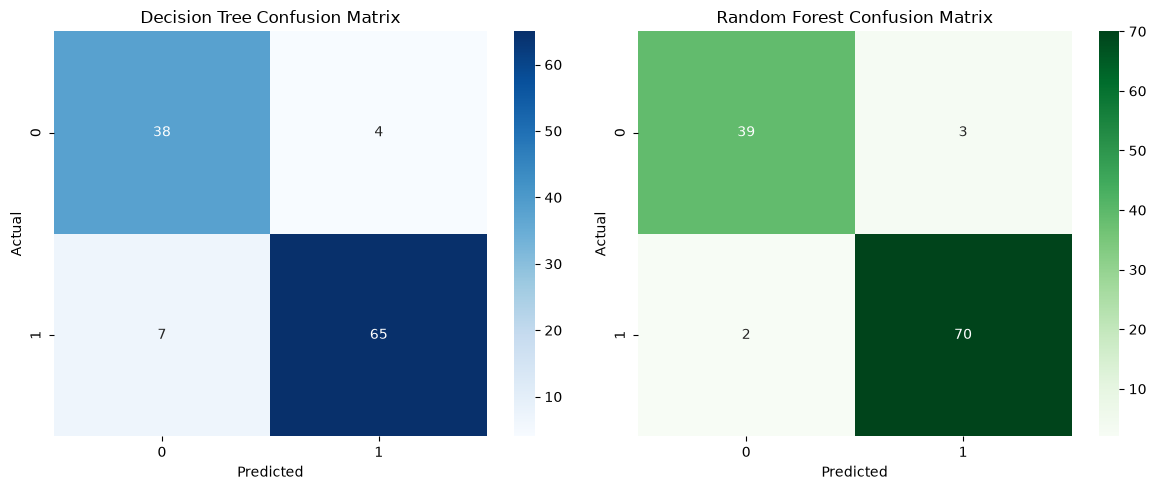
\includegraphics[width=0.85\linewidth]{images/confusion_matrix.png}
\caption{Confusion Matrices for Tuned Decision Tree and Random Forest Models}
\label{fig:confusion_matrices}
\end{figure}

\textbf{Inference:}
The confusion matrices indicate that both models exhibit strong classification performance on the test set of 114 samples (42 Malignant, 72 Benign). The tuned Decision Tree correctly classifies 65 Benign and 38 Malignant instances, producing 4 False Positives and 7 False Negatives. The tuned Random Forest correctly identifies 70 Benign and 39 Malignant instances, reducing False Positives to 3 and False Negatives to only 2. The significant reduction in classification errors (from 11 down to 5) highlights the effectiveness of ensemble learning in reducing variance and improving prediction boundaries.

\subsection{ROC Curves and AUC}
\begin{figure}[H]
\centering
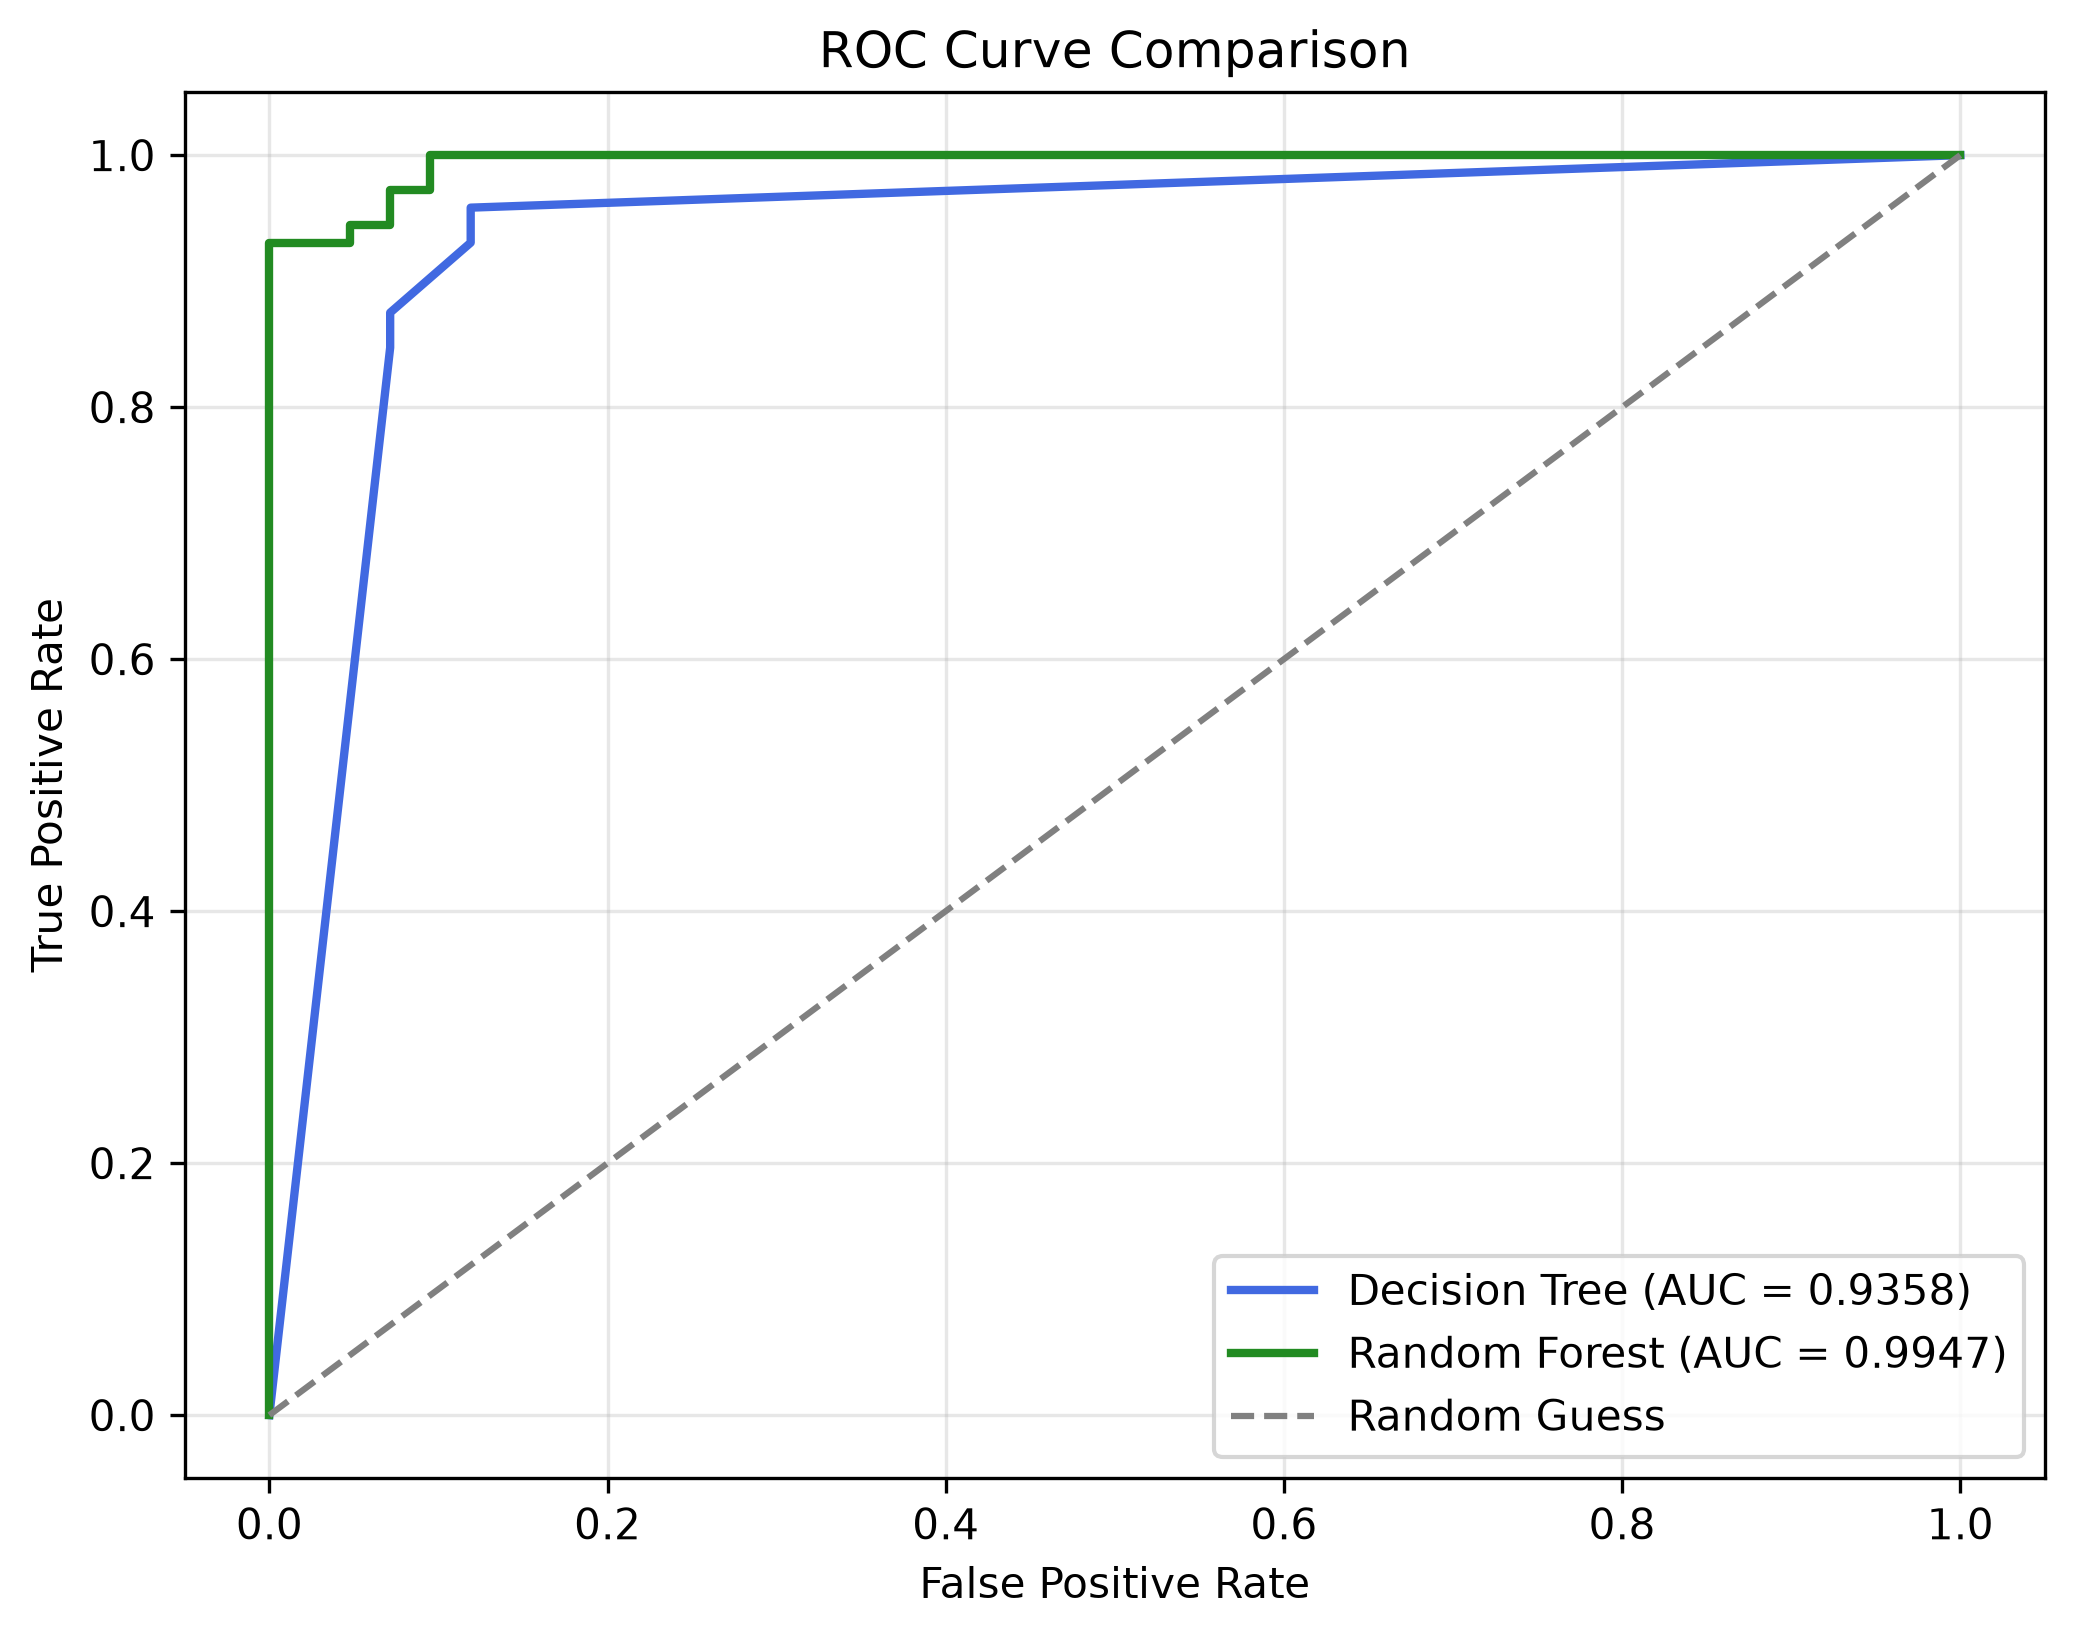
\includegraphics[width=0.7\linewidth]{images/roc_curve.png}
\caption{ROC Curve Comparison of Tuned Decision Tree and Random Forest}
\label{fig:roc_curve}
\end{figure}

\textbf{Inference:}
The Receiver Operating Characteristic (ROC) curve comparison displays the true positive rate against the false positive rate across different classification thresholds. The tuned Random Forest model achieves a near-perfect Area Under the Curve (AUC) of 0.9947, outperforming the tuned Decision Tree which obtains an AUC of 0.9358. This indicates that Random Forest is highly capable of ranking positive cases above negative cases, providing superior clinical utility by minimizing false negatives and false positives over a wide range of operational thresholds.

\section{Discussion}

\subsection{Best-Performing Classifier}
Based on the test set evaluations (Table~\ref{tab:test_results}), the \textbf{Tuned Random Forest} classifier significantly outperforms the \textbf{Tuned Decision Tree} classifier across all evaluation metrics. It achieves a test accuracy of \textbf{95.61\%} and F1-score of \textbf{0.9655}, compared to the Decision Tree's test accuracy of \textbf{90.35\%} and F1-score of \textbf{0.9220}. This represents a substantial decrease in classification error. The cross-validation performance (Table~\ref{tab:cv_acc_comp}) confirms this, as Random Forest achieves a consistently higher average validation accuracy of \textbf{96.48\%} compared to the Decision Tree's \textbf{93.85\%}, establishing Random Forest as a more stable and accurate model.

\subsection{Observation Questions}
\begin{enumerate}
    \item \textbf{How does tree depth affect overfitting in Decision Trees?}\\
    Tree depth directly regulates the complexity of the decision boundary. A shallow tree (e.g., depth 3) has high bias but low variance, occasionally underfitting the data. As tree depth increases, the model creates complex boundaries, split-rules, and leaf nodes containing very few samples to perfectly fit the training data. This drives the training error to zero but causes overfitting to noise, which degrades generalization on unseen test data. In our grid search, restricting the maximum depth to 5 and requiring at least 4 samples per leaf node acted as a form of pruning that stabilized validation performance.
    
    \item \textbf{Which hyperparameter had the greatest impact on performance?}\\
    For the Decision Tree, the splitting criterion and maximum depth had the greatest impact. The Gini criterion consistently outperformed Entropy at almost all depths, and limiting the tree depth to 5 was crucial to prevent overfitting. For the Random Forest, the choice of the maximum number of features considered at each split (\texttt{max\_features}) had the most significant impact. Restricting \texttt{max\_features} to \texttt{'log2'} ($\log_2(30) \approx 5$ features) yielded the best average CV F1-score (0.9720), consistently outperforming the configurations that used \texttt{'sqrt'} features ($\sqrt{30} \approx 5.5$ features). Limiting features at each node split forces individual trees to rely on different subsets of predictors, increasing ensemble diversity.
    
    \item \textbf{How does Random Forest improve generalization?}\\
    Random Forest improves generalization by constructing an ensemble of de-correlated decision trees. It implements two main techniques: Bagging (bootstrap aggregation) and Random Feature Selection. Each tree is trained on a distinct bootstrap sample of the training data. Additionally, at each node, only a random subset of features is evaluated for splitting. This sample and feature randomization ensures that individual trees develop different decision structures. While any individual tree may overfit its bootstrapped dataset, averaging their predictions cancels out the uncorrelated errors and variance of individual trees, leaving the overall bias unchanged but significantly reducing the ensemble's variance.
    
    \item \textbf{Did ensemble learning always improve performance? Why or why not?}\\
    Yes, ensemble learning consistently improved classification performance. The tuned Random Forest achieved superior metrics across all test set evaluations: higher accuracy (95.61\% vs. 90.35\%), precision (95.89\% vs. 94.20\%), recall (97.22\% vs. 90.28\%), F1-score (96.55\% vs. 92.20\%), and ROC-AUC (0.9947 vs. 0.9358). This occurs because the breast cancer dataset contains high-dimensional, highly correlated features. A single decision tree relies on a single deterministic partition tree that is highly sensitive to training partition variance. By utilizing 200 de-correlated trees, Random Forest smooths out decision boundaries, suppresses multicollinearity noise, and produces highly robust predictions.
\end{enumerate}

\section{Conclusion}
In this experiment, a single Decision Tree classifier and a Random Forest ensemble model were implemented, tuned, and evaluated on the Wisconsin Diagnostic Breast Cancer dataset. Hyperparameter optimization using 5-Fold Cross-Validation successfully identified the optimal configurations: a Decision Tree utilizing Gini impurity, max depth of 5, and min leaf samples of 4; and a Random Forest consisting of 200 estimators, max depth of 10, utilizing \texttt{'log2'} features without bootstrapping. 

The evaluation confirmed that Random Forest significantly outperformed the single Decision Tree, achieving a test accuracy of \textbf{95.61\%} and an ROC-AUC of \textbf{0.9947}, compared to the Decision Tree's \textbf{90.35\%} accuracy and \textbf{0.9358} AUC. These findings demonstrate that ensemble methods successfully address the high-variance limitations of individual decision trees, offering a highly robust and clinical-grade solution for breast cancer diagnosis.

\section{References}
\begin{enumerate}[label={[\arabic*]}]
    \item Scikit-learn Documentation. \textit{Decision Trees}. \url{https://scikit-learn.org/stable/modules/tree.html}
    \item Scikit-learn Documentation. \textit{Forests of randomized trees}. \url{https://scikit-learn.org/stable/modules/ensemble.html#forests-of-randomized-trees}
    \item UCI Machine Learning Repository. \textit{Breast Cancer Wisconsin (Diagnostic) Dataset}. \url{https://archive.ics.uci.edu/ml/datasets/Breast+Cancer+Wisconsin+(Diagnostic)}
    \item Breiman, L. (2001). \textit{Random Forests}. Machine Learning, 45(1), 5-32.
    \item Quinlan, J. R. (1986). \textit{Induction of Decision Trees}. Machine Learning, 1(1), 81-106.
\end{enumerate}

\end{document}
